\documentclass[11pt,a4paper]{article}
%%%%%%%%%%%%%%%%%%%%%%%%% Credit %%%%%%%%%%%%%%%%%%%%%%%%

% template ini dibuat oleh martin.manullang@if.itera.ac.id untuk dipergunakan oleh seluruh sivitas akademik itera.

%%%%%%%%%%%%%%%%%%%%%%%%% PACKAGE starts HERE %%%%%%%%%%%%%%%%%%%%%%%%
\usepackage{graphicx}
\usepackage{caption}
\usepackage{microtype}
\captionsetup[table]{name=Tabel}
\captionsetup[figure]{name=Gambar}
\usepackage{tabulary}
\usepackage{minted}
% \usepackage{amsmath}
\usepackage{fancyhdr}
% \usepackage{amssymb}
% \usepackage{amsthm}
\usepackage{placeins}
% \usepackage{amsfonts}
\usepackage{graphicx}
\usepackage[all]{xy}
\usepackage{tikz}
\usepackage{verbatim}
\usepackage[left=2cm,right=2cm,top=3cm,bottom=2.5cm]{geometry}
\usepackage{hyperref}
\hypersetup{
    colorlinks,
    linkcolor={red!50!black},
    citecolor={blue!50!black},
    urlcolor={blue!80!black}
}
\usepackage{caption}
\usepackage{subcaption}
\usepackage{multirow}
\usepackage{psfrag}
\usepackage[T1]{fontenc}
\usepackage[scaled]{beramono}
% Enable inserting code into the document
\usepackage{listings}
\usepackage{xcolor} 
% custom color & style for listing
\definecolor{codegreen}{rgb}{0,0.6,0}
\definecolor{codegray}{rgb}{0.5,0.5,0.5}
\definecolor{codepurple}{rgb}{0.58,0,0.82}
\definecolor{backcolour}{rgb}{0.95,0.95,0.92}
\definecolor{LightGray}{gray}{0.9}
\lstdefinestyle{mystyle}{
	backgroundcolor=\color{backcolour},   
	commentstyle=\color{green},
	keywordstyle=\color{codegreen},
	numberstyle=\tiny\color{codegray},
	stringstyle=\color{codepurple},
	basicstyle=\ttfamily\footnotesize,
	breakatwhitespace=false,         
	breaklines=true,                 
	captionpos=b,                    
	keepspaces=true,                 
	numbers=left,                    
	numbersep=5pt,                  
	showspaces=false,                
	showstringspaces=false,
	showtabs=false,                  
	tabsize=2
}
\lstset{style=mystyle}
\renewcommand{\lstlistingname}{Kode}
%%%%%%%%%%%%%%%%%%%%%%%%% PACKAGE ends HERE %%%%%%%%%%%%%%%%%%%%%%%%


%%%%%%%%%%%%%%%%%%%%%%%%% Data Diri %%%%%%%%%%%%%%%%%%%%%%%%
\newcommand{\student}{\textbf{Joshua Palti Sinaga(122140141), Irma Amelia Novianti(122140128)}}
\newcommand{\course}{\textbf{Pengolahan Sinyal Digital (IF3024)}}
\newcommand{\assignment}{\textbf{Tugas Besar}}

%%%%%%%%%%%%%%%%%%% using theorem style %%%%%%%%%%%%%%%%%%%%
\newtheorem{thm}{Theorem}
\newtheorem{lem}[thm]{Lemma}
\newtheorem{defn}[thm]{Definition}
\newtheorem{exa}[thm]{Example}
\newtheorem{rem}[thm]{Remark}
\newtheorem{coro}[thm]{Corollary}
\newtheorem{quest}{Question}[section]
%%%%%%%%%%%%%%%%%%%%%%%%%%%%%%%%%%%%%%%%
\usepackage{lipsum}%% a garbage package you don't need except to create examples.
\usepackage{fancyhdr}
\pagestyle{fancy}
\lhead{Joshua Palti Sinaga (122140141), Irma Amelia Novianti (22140128)}
\rhead{ \thepage}
\cfoot{\textbf{Detection Heart Rate and Respiration Rate}}
\renewcommand{\headrulewidth}{0.4pt}
\renewcommand{\footrulewidth}{0.4pt}

%%%%%%%%%%%%%%  Shortcut for usual set of numbers  %%%%%%%%%%%

\newcommand{\N}{\mathbb{N}}
\newcommand{\Z}{\mathbb{Z}}
\newcommand{\Q}{\mathbb{Q}}
\newcommand{\R}{\mathbb{R}}
\newcommand{\C}{\mathbb{C}}
\setlength\headheight{14pt}

%%%%%%%%%%%%%%%%%%%%%%%%%%%%%%%%%%%%%%%%%%%%%%%%%%%%%%%555
\begin{document}
\thispagestyle{empty}
\begin{center}
	\includegraphics[scale = 0.15]{Figure/ifitera-header.png}
	\vspace{0.1cm}
\end{center}
\noindent
\rule{17cm}{0.2cm}\\[0.3cm]
Nama: \student \hfill \\ 
Tugas Ke: \assignment\\[0.1cm]
Mata Kuliah: \course \hfill Tanggal: 31 Mei 2025\\
\rule{17cm}{0.05cm}
\vspace{0.1cm}



%%%%%%%%%%%%%%%%%%%%%%%%%%%%%%%%%%%%%%%%%%%%% BODY DOCUMENT %%%%%%%%%%%%%%%%%%%%%%%%%%%%%%%%%%%%%%%%%%%%%
\section{Deskripsi Projek}
    Proyek bertujuan untuk mendeteksi dan mengukur sinyal respirasi (pernapasan) dan sinyal detak jantung (rPPG - remote photoplethysmography) secara real-time menggunakan kamera webcam. Sistem ini dibangun dengan bahasa pemrograman Python dan menggabungkan berbagai teknologi seperti OpenCV untuk pemrosesan video, MediaPipe untuk deteksi wajah, serta algoritma POS (Plane-Orthogonal-to-Skin) untuk ekstraksi sinyal rPPG dari perubahan warna pada wajah. Sinyal respirasi diperoleh melalui analisis gerakan bahu pengguna, sementara sinyal detak jantung dihitung berdasarkan sinyal RGB yang difilter dan dianalisis menggunakan transformasi Fourier. Sistem ini juga dilengkapi fitur deteksi manual untuk membandingkan estimasi sinyal otomatis dengan input pengguna secara langsung.

\section{Teknologi}
    Teknologi yang digunakan dalam mengerjakan Final Project ini adalah sebagai berikut : 
    \begin{itemize}
        \item Python adalah bahasa pemrograman tinggat tinggi dan memiliki sintaks yang sederhana serta library yang memudahkan dalam membuat program, termasuk untuk mengolah gambar, video dan data.
        \item OpenCV adalah library yang digunakan untuk memproses gambar dan video seperti mengenali wajah atau melacak gerakan objek dari kamera dan bekerja secara real-time.
        \item MediaPipe adalah teknologi yang bisa mengenali dan melacak bagian tubuh manusia seperti wajah, tangan, dan gerakan tubuh dari video.
        \item POS (Plane-Orthogonal-to-Skin) adalah metode untuk mendeteksi detak jantung dari video wajah dengan cara mengolah informasi tentang perubahan intensitas warna RGB pada area wajah, dan memisahkan sinyal penting dari gangguan cahaya atau gerakan.
    \end{itemize}

\section{Cara Kerja}
    Sistem ini bekerja dengan memanfaatkan webcam untuk menangkap video pengguna secara real-time. Setiap frame dari video yang ditangkap diproses untuk deteksi wajah menggunakan teknologi MediaPipe Face Detection. Kemudian dilakukan tracking menggunakan metode Lucas-Kanade dengan cara mencari titik-titik lankmark pada wajah. Dari titik-titik ini, sistem menentukan area tertentu pada wajah (Region of Interest/ROI) untuk mengambil nilai rata-rata warna RGB. Nilai-nilai RGB ini kemudian digunakan dalam algoritma POS (Plane-Orthogonal-to-Skin) yang mengubahnya menjadi sinyal rPPG, yang kemudian difilter menggunakan filter bandpass dan dianalisis oleh FFT (Fast Fourier Transform) untuk menghitung perkiraan denyut jantung dalam BPM (beats per minute).

    Sistem ini juga mendeteksi gerakan bahu dari posisi vertikal dalam frame video. Nilai-nilai perubahan posisi ini diproses menjadi sinyal pernapasan yang juga difilter dan dianalisis untuk mendapatkan frekuensi napas dalam BPM. Selain metode otomatis ini, sistem menyediakan fitur input manual, di mana pengguna dapat menekan tombol saat merasakan detak nadi atau bernapas. Data waktu ketukan ini digunakan untuk menghitung BPM manual sebagai perbandingan terhadap hasil dari proses otomatis. Semua hasil pemrosesan sinyal ditampilkan secara visual melalui antarmuka atau grafik, untuk pemantauan detak jantung dan pernapasan.

\section{Analisis Matematis Filter yang Digunakan}
Sistem ini menggunakan empat jenis filter sinyal digital untuk membersihkan dan memproses sinyal rPPG dan respirasi secara real-time. Setiap filter memiliki berfungsi untuk mengurangi noise dan mendapatkan sinyal yang diharapkan.

\subsection{Filter Butterworth Bandpass}
Filter Butterworth Bandpass adalah filter yang hanya membolehkan frekuensi dalam rentang tertentu sambil memblokir frekuensi di luar rentang tersebut \cite{scipy2024}. Filter ini berguna untuk memisahkan sinyal detak jantung dari noise lain seperti gerakan tubuh atau perubahan pencahayaan.

\subsubsection{Rumus dan Implementasi}
    \begin{lstlisting}
def bandpass_filter(self, data, low_freq, high_freq):
    data_array = np.array(list(data)[-60:])
    nyquist = self.fps / 2  # = 15 Hz untuk fps=30
    low = low_freq / nyquist
    high = high_freq / nyquist
    
    b, a = signal.butter(3, [low, high], btype='band')
    filtered = signal.filtfilt(b, a, data_array)
    return filtered[-1]
    \end{lstlisting}

\subsubsection{Parameter Filter untuk Heart Rate}
Untuk sinyal rPPG (heart rate), sistem menggunakan:
\begin{itemize}
    \item \textbf{Orde filter}: $N = 3$ (filter Butterworth orde 3)
    \item \textbf{Frekuensi cutoff bawah}: $f_{low} = 0.8$ Hz (48 BPM)
    \item \textbf{Frekuensi cutoff atas}: $f_{high} = 2.8$ Hz (168 BPM)
    \item \textbf{Frekuensi Nyquist}: $f_{nyq} = \frac{f_s}{2} = \frac{20}{2} = 10$ Hz
\end{itemize}

Frekuensi normalisasi yang digunakan:
$$\omega_{low} = \frac{f_{low}}{f_{nyq}} = \frac{0.8}{15} = 0.8$$
$$\omega_{high} = \frac{f_{high}}{f_{nyq}} = \frac{2.8}{10} = 0.28$$
Frekuensi normalisasi merupakan frekuensi yang dinormalisasi menjadi rentang frekuensi antara  0 hingga 1, dimana 1 adalah frekuensi Nyquist. Parameter ini diperlukan agar filter dapat bekerja konsisten tanpa terpengaruh oleh sampling rate.

\subsubsection{Parameter Filter untuk Respiration Rate}
Untuk sinyal respirasi, sistem menggunakan:
\begin{itemize}
    \item \textbf{Orde filter}: $N = 3$
    \item \textbf{Frekuensi cutoff bawah}: $f_{low} = 0.1$ Hz (6 RPM)
    \item \textbf{Frekuensi cutoff atas}: $f_{high} = 0.8$ Hz (48 RPM)
\end{itemize}

Frekuensi normalisasi:
$$\omega_{low} = \frac{0.1}{10} = 0.01$$
$$\omega_{high} = \frac{0.8}{10} = 0.08$$


\subsection{Filter Savitzky-Golay}
Filter Savitzky-Golay adalah filter penghalus (smoothing filter) yang menggunakan teknik fitting polinomial untuk mengurangi noise tanpa merusak bentuk asli sinyal. Filter ini sangat baik untuk mempertahankan puncak dan lembah sinyal yang penting untuk deteksi detak jantung \cite{savitzky1964}.
Filter ini bekerja dengan mengambil sejumlah titik data di sekitar setiap sampel, kemudian mencocokkan kurva polinomial melalui titik-titik tersebut. Nilai yang dihaluskan adalah nilai polinomial pada titik tengah. Proses ini dilakukan untuk setiap sampel, sehingga menghasilkan sinyal yang lebih halus tapi tetap mempertahankan karakteristik penting.

\subsubsection{Rumus dan Implementasi}
    \begin{lstlisting}
def apply_savgol_filter(self, data, window_length=11, polyorder=3):
    data_array = np.array(list(data)[-window_length:])
    filtered = savgol_filter(data_array, window_length, polyorder)
    return filtered[-1]
    \end{lstlisting}

Rumus dasar Savitzky-Golay:
$$y_{smoothed}[i] = \sum_{j=-m}^{m} C_j \cdot y[i+j]$$

dimana $C_j$ adalah koefisien yang dihitung dari fitting polinomial dan $m = \frac{window\_length-1}{2}$.

\subsubsection{Parameter yang Digunakan}
\begin{itemize}
    \item \textbf{Heart Rate Signal}: Window length = 14, Polynomial order = 4
\end{itemize}

\subsection{Moving Average Filter}
Moving average filter adalah filter yang menghitung rata-rata dari sejumlah titik data berturut-turut. Filter ini efektif untuk mereduksi noise frekuensi tinggi \cite{smith1997} . Filter ini digunakan untuk menghaluskan sinyal dari bahu sebelum analisis respirasi, mereduksi fluktuasi cepat yang diakbatkan oleh gerakan kecil atau noise. Pada sistem, filter ini mengambil 15 sampel di sekitar setiap titik data (7 sebelumnya, titik saat ini, dan 7 sesudahnya), kemudian menghitung rata-ratanya. Filter ini membuat sinyal lebih halus dan menghilangkan perubahan cepat yang tidak relevan untuk deteksi respirasi.

\subsubsection{Rumus dan Implementasi}
    \begin{lstlisting}
# Moving window smoothing dengan window size = 15
for i in range(len(y_window)):
    start_idx = max(0, i - self.shoulder_smoothing_window // 2)
    end_idx = min(len(y_window), i + self.shoulder_smoothing_window // 2 + 1)
    smoothed_window.append(np.mean(y_window[start_idx:end_idx]))
    \end{lstlisting}

Rumus centered moving average:
$$y[n] = \frac{1}{N} \sum_{k=-\frac{N-1}{2}}^{\frac{N-1}{2}} x[n+k]$$

dimana $N = 15$ adalah ukuran window.

\subsubsection{Parameter yang Digunakan}
\begin{itemize}
    \item \textbf{Window size}: 15 sampel
\end{itemize}

\subsection{Windowing untuk FFT Analysis (Hanning Window)}
Hanning window adalah fungsi jendela berbasis kosinus yang digunakan sebelum FFT ( Fast Fourier Transform) untuk mengurangi efek spectral leakage akibat pemotongan sinyal. Dengan meredam nilai sinyal di awal dan akhir segmen, window ini membantu menghasilkan spektrum frekuensi yang lebih akurat dan bersih \cite{scipy2024}. 

\subsubsection{Rumus dan Implementasi}
    \begin{lstlisting}
def estimate_heart_rate(self):
    data = np.array(list(self.pos_savgol_buffer)[-150:])
    data = data - np.mean(data)
    windowed = data * np.hanning(len(data))  # Aplikasi Hanning window
    fft_vals = np.abs(np.fft.fft(windowed))
    \end{lstlisting}

Rumus Hanning window:
$$w[n] = 0.5 \left(1 - \cos\left(\frac{2\pi n}{N-1}\right)\right)$$

dimana $n = 0, 1, 2, ..., N-1$ dan $N$ adalah panjang window.

\subsubsection{Parameter yang Digunakan}
\begin{itemize}
    \item \textbf{Window length}: 150 sampel untuk heart rate, 180 sampel untuk respiration
\end{itemize}


\section{Implementasi Program}

\subsection{Mendownload seluruh isi project dari GitHub ke komputer lokal}
    \begin{itemize}
        \item Buka terminal atau command prompt
        \item Jalankan perintah berikut : 
        \begin{lstlisting}
        git clone https://github.com/jo0707/dsp-realtime-rppg-respiration.git\end{lstlisting}
        \item Masuk ke dalam direktori proyek 
        \begin{lstlisting}
            cd dsp-realtime-rppg-respiration\end{lstlisting}
    \end{itemize}
    Perintah git clone akan menyalin semua file dari repositori ke folder lokal, lalu perintah cd digunakan untuk masuk ke dalam direktori proyek tersebut.

\subsection{Buat dan aktifkan virtual environment (Opsional)}
    \begin{itemize}
        \item Untuk Linux/Mac : 
        \begin{lstlisting}
            uv venv
            source venv/bin/activate\end{lstlisting}
        \item Untuk Windows
        \begin{lstlisting}
            uv venv
            .venv\Scripts\activate\end{lstlisting}\end{itemize}
    Aktifkan virtual environment agar paket python yang digunnakan tidak bercampur dengan sistem global. Virtual environment adalah lingkungan Python terpisah, yang membantu mencegah konflik antar proyek.
    
\subsection{Install Semua Depedency}
    Setelah environment aktif, instal semua paket yang dibutuhkan dengan menjalankan:
    \begin{lstlisting}
        pip install -r requirements.txt

        uv pip install -r requirements.txt // jika menggunakan uv\end{lstlisting}
    Perintah ini akan membaca file requirements.txt dan menginstal semua library seperti opencv-python, numpy, mediapipe, dan lainnya yang diperlukan program agar bisa berjalan.

\subsection{Jalankan Program}
    \begin{lstlisting}
        python main.py\end{lstlisting}
    File main.py akan menjalankan program secara real-time
    Rekan tombol start untuk memulai program
    \begin{figure}[h]
    \centering
    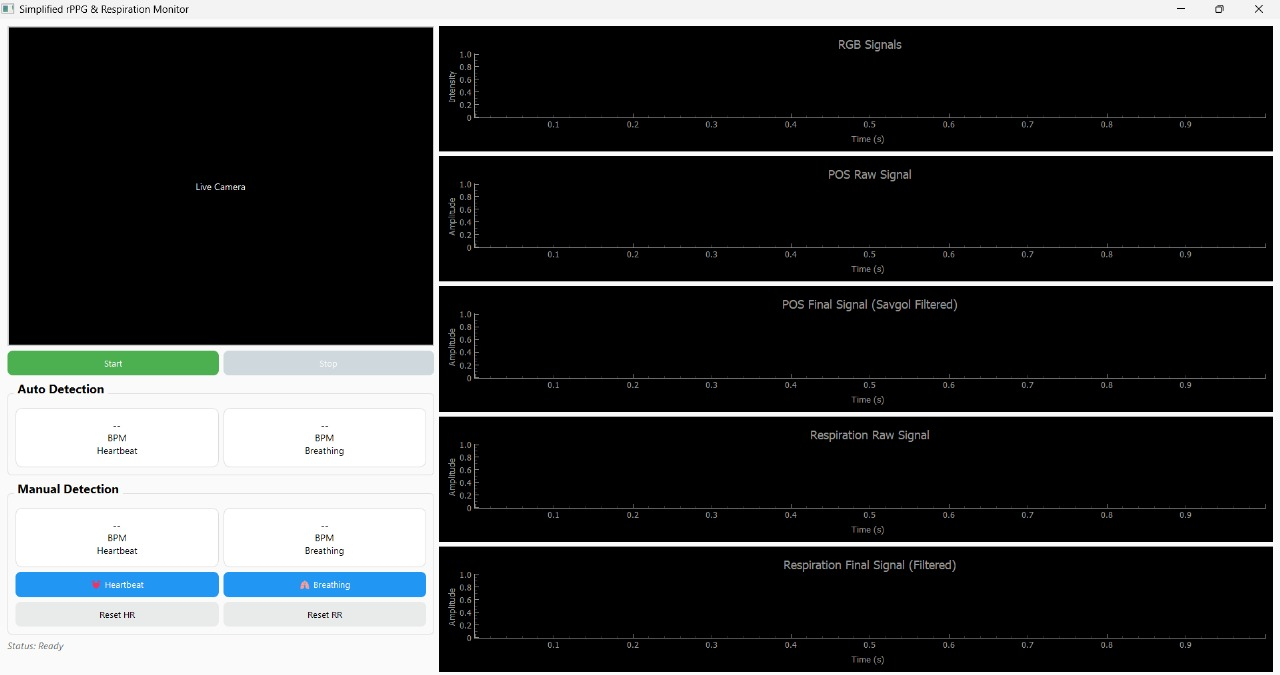
\includegraphics[width=0.8\textwidth]{Figure/ready.jpg}
    \caption{Tampilan sebelum start}
    \label{fig:my_label}
    \end{figure}
    \begin{figure}[h]
    \centering
    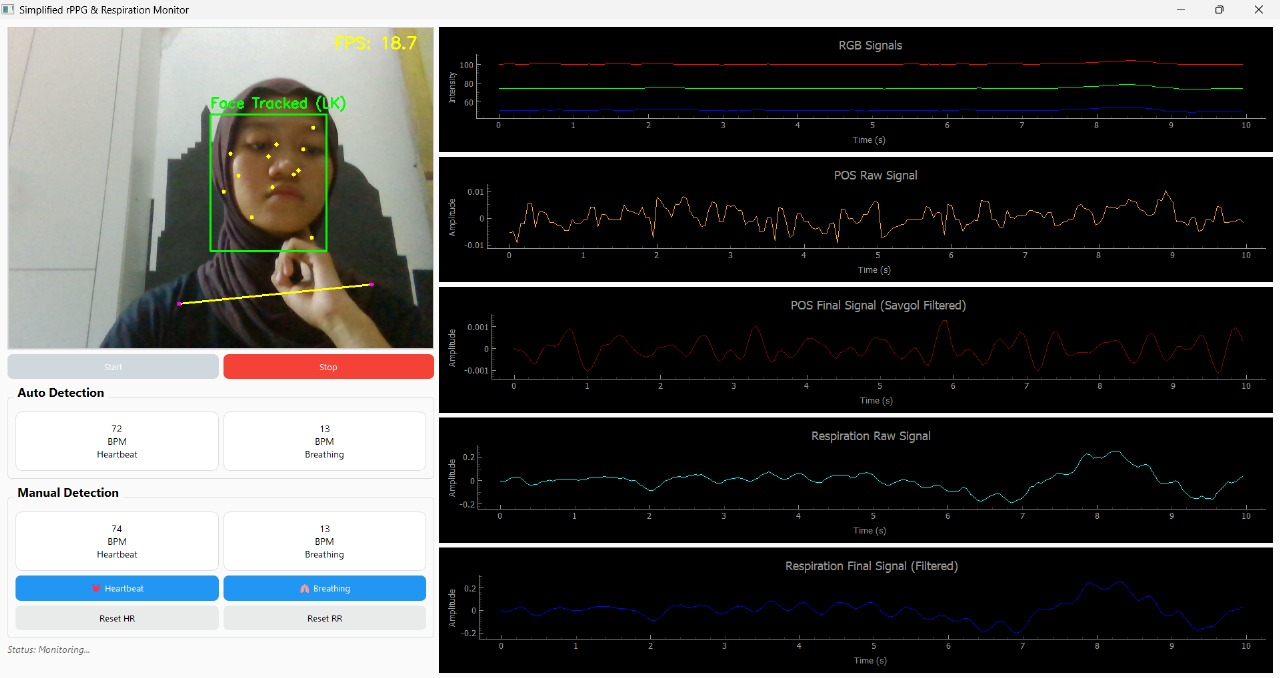
\includegraphics[width=0.8\textwidth]{Figure/monitoring.jpg}
    \caption{Tampilan ketika program berjalan}
    \label{fig:my_label}
    \end{figure}
    
    \begin{itemize}
        \item Sistem akan mulai melakukan perhitungan estimasi rPPG dan pernafasan.
        \item sistem menyediakan fitur input manual, di mana pengguna dapat menekan tombol saat merasakan detak nadi atau bernapas
        \item Semua hasil pemrosesan sinyal ditampilkan secara visual melalui antarmuka atau grafik, untuk pemantauan detak jantung dan pernapasan.
    \end{itemize}


\section{Alur Pemrosesan Sinyal}

\subsection{Inisialisasi Sistem dan Pengaturan FPS}
    \begin{lstlisting}
def main():
    app = QApplication(sys.argv)
    fps = 20
    buffer_size = 200
    
    camera_processor = CameraProcessor(fps=fps)
    signal_processor = SignalProcessor(fps=fps, buffer_size=buffer_size)
    
    window = MainWindow(camera_processor, signal_processor)
    window.show()
    \end{lstlisting}
    Sistem dimulai dengan inisialisasi komponen utama: CameraProcessor untuk pengolahan video, SignalProcessor untuk analisis sinyal, dan MainWindow untuk antarmuka pengguna. Parameter FPS diset ke 20 dan buffer size 200 untuk optimasi performa real-time.

\subsection{Pengambilan Frame dari Webcam dengan GUI}
    \begin{lstlisting}
def start_monitoring(self):
    self.cap = cv2.VideoCapture(0)
    self.cap.set(cv2.CAP_PROP_FPS, self.camera_processor.fps)
    self.timer.start(33)  # ~30 FPS
    self.start_btn.setEnabled(False)
    self.stop_btn.setEnabled(True)
    self.status_label.setText("Status: Monitoring...")
    \end{lstlisting}
    Proses monitoring dimulai ketika tombol "Start" ditekan. Sistem menggunakan QTimer dengan interval 33ms untuk mencapai ~30 FPS dalam pemrosesan frame. Status GUI diperbarui untuk menunjukkan sistem sedang aktif.

\subsection{Deteksi Wajah dengan MediaPipe dan Lucas-Kanade Tracking}
    \begin{lstlisting}
def detect_face_initial(self, frame):
    rgb_frame = cv2.cvtColor(frame, cv2.COLOR_BGR2RGB)
    results = self.face_detection.process(rgb_frame)
    
    if results.detections:
        detection = results.detections[0]
        bbox = detection.location_data.relative_bounding_box
        # Definisi area dahi (forehead region)
        forehead_y = y + int(height * 0)
        forehead_height = int(height * 0.9)
        forehead_x = x + int(width * 0.1)
        forehead_width = int(width * 0.7)
        
        # Buat grid tracking points di area dahi
        key_points = []
        for i in range(points_per_col):
            for j in range(points_per_row):
                px = forehead_x + (j * forehead_width // (points_per_row - 1))
                py = forehead_y + (i * forehead_height // (points_per_col - 1))
                key_points.append([px, py])
    \end{lstlisting}
    Deteksi wajah awal menggunakan MediaPipe untuk menentukan bounding box wajah. Sistem membuat grid 4x3 tracking points pada area dahi (90% dari tinggi wajah, 70% dari lebar wajah) yang akan digunakan untuk Lucas-Kanade tracking.

\subsection{Tracking Wajah dengan Lucas-Kanade Optical Flow}
    \begin{lstlisting}
def track_face_lk(self, frame):
    gray = cv2.cvtColor(frame, cv2.COLOR_BGR2GRAY)
    
    new_points, status, error = cv2.calcOpticalFlowPyrLK(
        self.prev_gray, gray, self.face_points, None, **self.lk_params)
    
    status = status.flatten()
    good_new = new_points[status == 1]
    
    if len(good_new) < 6:
        return None  # Tracking gagal, perlu re-detection
        
    self.face_points = good_new.reshape(-1, 1, 2)
    self.prev_gray = gray.copy()
    \end{lstlisting}
    Setelah deteksi awal, sistem menggunakan Lucas-Kanade optical flow untuk tracking yang lebih efisien. Parameter tracking: winSize=(15,15), maxLevel=2, criteria berdasarkan EPS dan COUNT. Jika kurang dari 6 points yang valid, sistem kembali ke re-detection.

\subsection{Ekstraksi Sinyal RGB dari Area Wajah}
    \begin{lstlisting}
def detect_face(self, frame):
    # ...existing tracking code...
    
    face_region = frame[y_min:y_max, x_min:x_max]
    if face_region.size > 0:
        b_mean = np.mean(face_region[:, :, 0])
        g_mean = np.mean(face_region[:, :, 1])
        r_mean = np.mean(face_region[:, :, 2])
        
        # Visualisasi tracking
        cv2.rectangle(frame, (x_min, y_min), (x_max, y_max), (0, 255, 0), 2)
        for point in self.face_points:
            x, y = point.ravel()
            cv2.circle(frame, (int(x), int(y)), 3, (0, 255, 255), -1)
            
        return r_mean, g_mean, b_mean
    \end{lstlisting}
    Dari area wajah yang berhasil di-track, sistem menghitung nilai rata-rata RGB. Area ini divisualisasikan dengan rectangle hijau dan tracking points kuning pada GUI real-time.

\subsection{Penyimpanan Sinyal RGB ke Buffer}
    \begin{lstlisting}
def process_rgb_signal(self, r, g, b):
    if r is not None and not np.isnan(r) and not np.isnan(g) and not np.isnan(b):
        self.rgb_buffer.append([r, g, b])
        
        if len(self.rgb_buffer) >= self.min_window:
            recent_rgb = np.array(list(self.rgb_buffer)[-self.min_window:])
            recent_rgb = recent_rgb.T.reshape(1, 3, -1)
    \end{lstlisting}
    Nilai RGB yang valid (tidak None dan tidak NaN) disimpan dalam rgb\_buffer dengan ukuran maksimal 200 sampel. Minimum window untuk POS algorithm adalah 48 sampel (1.6 detik × 30 FPS).

\subsection{Algoritma POS (Plane-Orthogonal-to-Skin)}
    \begin{lstlisting}
def simple_pos_algorithm(self, signal):
    eps = 1e-9
    X = signal
    P = np.array([[0, 1, -1], [-2, 1, 1]], dtype=np.float64)
    
    for n in range(self.min_window-1, f):
        m = n - self.min_window + 1
        Cn = X[:, :, m:n+1]
        
        # Temporal normalization
        mean_vals = np.mean(Cn, axis=2, keepdims=True)
        mean_vals = np.where(mean_vals == 0, eps, mean_vals)
        Cn_normalized = Cn / mean_vals
        
        # Proyeksi ke POS space
        S = np.dot(P, rgb_window)
        
        # Tuning step
        alpha = std1 / std2 if std2 > eps else 1.0
        Hn = S1 + alpha * S2 - np.mean(S1 + alpha * S2)
        
        # Overlap-add
        heart_rate_signal[i, m:n+1] += Hn
    \end{lstlisting}
    Algoritma POS menggunakan sliding window untuk memproses sinyal RGB. Matriks proyeksi P=[0,1,-1; -2,1,1] memisahkan sinyal menjadi dua komponen ortogonal. Parameter alpha menyesuaikan kontribusi kedua komponen berdasarkan standar deviasi.

\subsection{Multi-Stage Filtering untuk Heart Rate}
    \begin{lstlisting}
# Stage 1: Bandpass Filter
pos_filtered = self.bandpass_filter(self.pos_raw_buffer, 
                                   self.heart_rate_low_freq, 
                                   self.heart_rate_high_freq)

# Stage 2: Savitzky-Golay Filter  
pos_savgol = self.apply_savgol_filter(self.pos_filtered_buffer, 14, 4)
self.pos_savgol_buffer.append(pos_savgol)
    \end{lstlisting}
    Sinyal POS melewati dua tahap filtering: (1) Butterworth bandpass filter orde-3 dengan range 0.8-2.8 Hz, (2) Savitzky-Golay filter dengan window=14 dan polynomial order=4 untuk smoothing akhir.

\subsection{Deteksi Bahu dengan MediaPipe Pose}
    \begin{lstlisting}
def detect_shoulders_initial(self, frame):
    rgb_frame = cv2.cvtColor(frame, cv2.COLOR_BGR2RGB)
    results = self.pose.process(rgb_frame)
    
    if results.pose_landmarks:
        landmarks = results.pose_landmarks.landmark
        left_shoulder = landmarks[11]  # Left shoulder landmark
        right_shoulder = landmarks[12] # Right shoulder landmark
        
        left_x, left_y = int(left_shoulder.x * w), int(left_shoulder.y * h)
        right_x, right_y = int(right_shoulder.x * w), int(right_shoulder.y * h)
        
        key_points = [[left_x, left_y], [right_x, right_y]]
        self.shoulder_points = np.array(key_points, dtype=np.float32)
    \end{lstlisting}
    MediaPipe Pose mendeteksi 33 landmark tubuh, sistem menggunakan landmark 11 (bahu kiri) dan 12 (bahu kanan). Re-deteksi dilakukan setiap 100 frame untuk akurasi tracking.

\subsection{Tracking Bahu dan Ekstraksi Sinyal Respirasi}
    \begin{lstlisting}
def track_shoulders_lk(self, frame):
    new_points, status, error = cv2.calcOpticalFlowPyrLK(
        self.shoulder_prev_gray, gray, self.shoulder_points, None, **self.lk_params)
    
    good_new = new_points[status.flatten() == 1]
    if len(good_new) < 2:
        return None
        
    left_shoulder = self.shoulder_points[0, 0]
    right_shoulder = self.shoulder_points[1, 0]
    mid_y = (left_y + right_y) // 2
    return mid_y
    \end{lstlisting}
    Tracking bahu menggunakan Lucas-Kanade dengan parameter yang sama seperti tracking wajah. Posisi Y tengah antara kedua bahu digunakan sebagai sinyal respirasi mentah.

\subsection{Moving Window Smoothing untuk Sinyal Respirasi}
    \begin{lstlisting}
def process_shoulder_signal(self, shoulder_y):
    if shoulder_y is not None:
        self.shoulder_buffer.append(shoulder_y)
        
        if len(self.shoulder_buffer) >= 30:
            y_window = np.array(list(self.shoulder_buffer)[-30:])
            
            # Moving window smoothing
            smoothed_window = []
            for i in range(len(y_window)):
                start_idx = max(0, i - self.shoulder_smoothing_window // 2)
                end_idx = min(len(y_window), i + self.shoulder_smoothing_window // 2 + 1)
                smoothed_window.append(np.mean(y_window[start_idx:end_idx]))
            
            movement = np.mean(np.gradient(smoothed_window))
            self.resp_raw_buffer.append(movement)
    \end{lstlisting}
    Sinyal bahu dihaluskan dengan moving window berukuran 15 sampel. Gradient dihitung untuk mendeteksi perubahan posisi yang mengindikasikan pernapasan.

\subsection{Estimasi Heart Rate dan Respiration Rate dengan FFT}
    \begin{lstlisting}
def estimate_heart_rate(self):
    data = np.array(list(self.pos_savgol_buffer)[-150:])
    data = data - np.mean(data)
    windowed = data * np.hanning(len(data))
    fft_vals = np.abs(np.fft.fft(windowed))
    freqs = np.fft.fftfreq(len(windowed), 1/self.fps)
    
    hr_mask = (freqs >= 0.8) & (freqs <= 2.8)
    peak_freq = freqs[hr_mask][np.argmax(fft_vals[hr_mask])]
    self.heart_rate = peak_freq * 60
    \end{lstlisting}
    FFT analysis menggunakan Hanning window untuk mengurangi spectral leakage. Heart rate dicari pada range 0.8-2.8 Hz, respiration rate pada range 0.1-0.8 Hz. Peak detection menentukan frekuensi dominan.

\subsection{Update GUI Real-time dan Visualisasi}
    \begin{lstlisting}
def update_frame(self):
    ret, frame = self.cap.read()
    if ret:
        processed_frame = self.camera_processor.process_frame(frame, self.signal_processor)
        
        # Update displays
        self.auto_hr_display.setText(f"{self.signal_processor.heart_rate:.0f}\\nBPM\\nHeartbeat")
        self.auto_rr_display.setText(f"{self.signal_processor.respiration_rate:.0f}\\nBPM\\nBreathing")
        
        # Update plots
        self.update_plots()
    \end{lstlisting}
    Setiap frame diproses dan hasilnya ditampilkan pada GUI. Lima plot real-time menunjukkan: (1) RGB signals, (2) POS raw, (3) POS filtered, (4) Respiration raw, (5) Respiration filtered.

\subsection{Deteksi Manual sebagai Ground Truth}
    \begin{lstlisting}
def tap_heartbeat(self):
    current_time = time.time()
    self.heartbeat_taps.append(current_time)
    
    if len(self.heartbeat_taps) >= 2:
        recent_taps = list(self.heartbeat_taps)[-10:]
        intervals = []
        for i in range(1, len(recent_taps)):
            interval = recent_taps[i] - recent_taps[i-1]
            if 0.3 <= interval <= 2.0:  # Valid heart rate range
                intervals.append(interval)
        
        if intervals:
            avg_interval = np.mean(intervals)
            self.manual_heart_rate = 60.0 / avg_interval
    \end{lstlisting}
    Pengguna dapat mengetuk tombol saat merasakan detak jantung atau napas. Sistem menghitung interval antar ketukan dan memvalidasi range fisiologis (0.3-2.0s untuk HR, 1.0-10.0s untuk RR) sebelum menghitung BPM manual sebagai pembanding.

\section{Analisis Hasil dan Pembahasan}

    \begin{figure}[h]
    \centering
    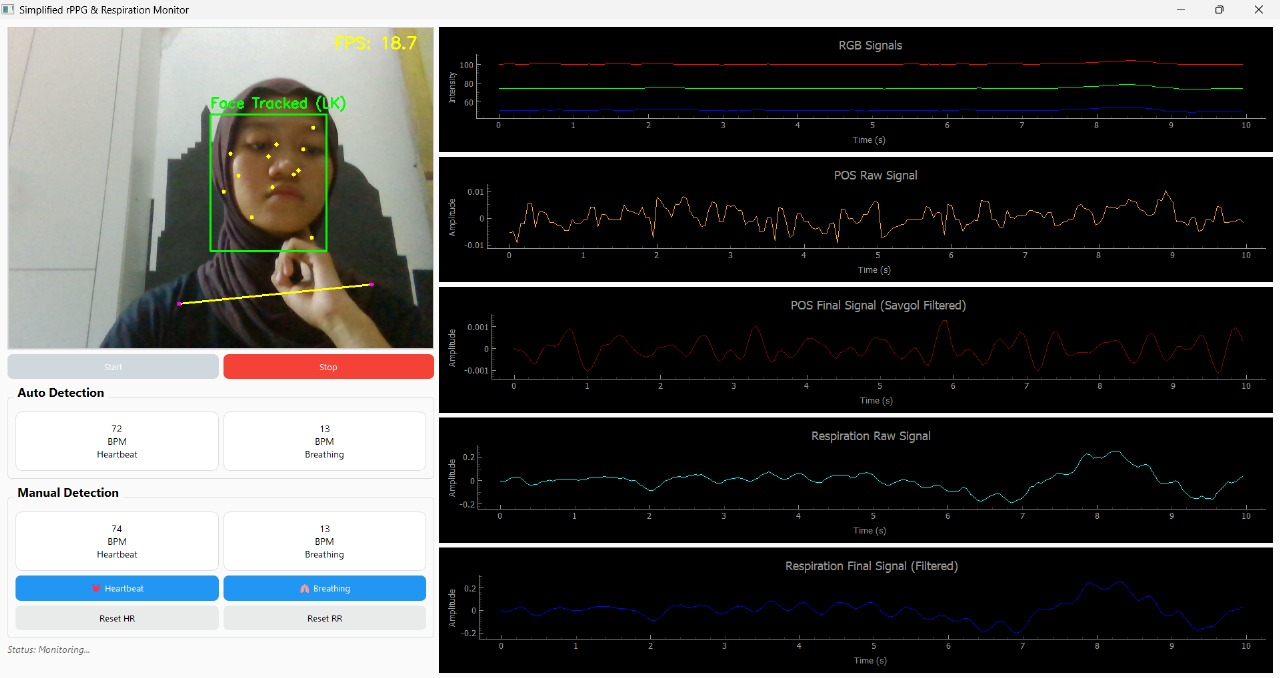
\includegraphics[width=0.8\textwidth]{Figure/monitoring.jpg}
    \caption{HR/RR}
    \label{fig:my_label}
    \end{figure}

\subsection{Hasil Deteksi Sinyal rPPG (Detak Jantung)}
    Sinyal rPPG (remote Photoplethysmography) diekstraksi dari area wajah pengguna berdasarkan perubahan nilai RGB. Proses ini dimulai dari pengambilan data warna kulit, dilanjutkan dengan ekstraksi sinyal menggunakan algoritma Plane-Orthogonal-to-Skin (POS), kemudian dilakukan filtrasi.
    Hasil visualisasi antarmuka menunjukkan:
    \begin{itemize}
    \item RGB Signals : Menampilkan intensitas warna merah, hijau, dan biru yang diperoleh dari ROI (Region of Interest) pada wajah. Fluktuasi mencerminkan variasi aliran darah.
    \item POS Raw Signal: Hasil sinyal setelah transformasi POS dari RGB. Masih mengandung noise.
    \item POS Final Signal (Savgol Filtered): Hasil dari dua tahap filtering, yaitu bandpass filter Butterworth dan filter Savitzky-Golay. Sinyal terlihat lebih halus dan periodik.
    \end{itemize}

Dari sinyal akhir POS, dilakukan Fast Fourier Transform (FFT) untuk mendapatkan frekuensi dominan, lalu dikonversi menjadi BPM (beats per minute). Diperoleh hasil untuk  Auto HR = 72 BPM dan Manual HR = 74 BPM. Perbedaan antara HR otomatis dan manual biasanya berada di bawah ±5 BPM, yang menunjukkan estimasi cukup akurat.

\subsection{2. Hasil Deteksi Sinyal Respirasi (Respiratory Rate)}
Sinyal pernapasan diperoleh dari gerakan vertikal bahu kiri dan kanan, ditentukan melalui posisi titik bahu dari MediaPipe Pose.

Hasil visualisasi antarmuka menunjukkan
\begin{itemize}
    \item Respiration Raw Signal : Dihasilkan dari perubahan posisi bahu, kemudian dihitung gradien perubahannya.
    \item Respiration Final Signal (Filtered) : Telah melalui moving average dan Savitzky-Golay filter untuk menghaluskan gelombang pernapasan.
    \end{itemize}

    Estimasi RR dilakukan dengan FFT pada sinyal respirasi yang telah difilter. Diperoleh hasil untuk Auto RR = 13 BPM, Manual RR = 13 BPM. Deteksi respirasi cenderung lebih sensitif terhadap noise akibat postur duduk yang tidak stabil atau gerakan mendadak.

\subsection{Deteksi Manual (Manual Tapping)}
    Pengguna dapat mendeteksi HR dan RR secara manual melalui tombol \texttt{Heartbeat} dan \texttt{Breathing}. Setiap ketukan menyimpan waktu (\textit{timestamp}) yang kemudian digunakan untuk menghitung rata-rata selisih waktu antar ketukan.

    Fitur ini bermanfaat untuk validasi terhadap hasil deteksi otomatis. Perbedaan antara manual dan otomatis bisa terjadi jika tapping tidak dilakukan secara konsisten atau saat pengguna tidak fokus.

\subsection{Pengaruh Filter Digital}
    Penggunaan filter Butterworth bandpass efektif dalam mengeliminasi noise frekuensi rendah (gerakan tubuh) dan noise frekuensi tinggi (fluktuasi acak) pada sinyal rPPG. Savitzky-Golay filter memberikan smoothing tambahan tanpa menghilangkan peak sinyal, sehingga deteksi frekuensi dominan oleh FFT menjadi lebih stabil. Pada sinyal respirasi, moving average filter berhasil meredam fluktuasi akibat noise tracking bahu, sehingga pola pernapasan lebih jelas terlihat pada plot.


\subsection{Kendala dan Faktor yang Mempengaruhi Akurasi}
Beberapa kendala yang ditemukan antara lain:
\begin{itemize}
    \item Pencahayaan: Intensitas cahaya yang terlalu rendah atau terlalu terang menyebabkan noise pada sinyal RGB, sehingga estimasi HR/RR menjadi kurang stabil.
    \item Gerakan Kepala/Bahu : Gerakan mendadak atau perubahan posisi wajah/bahu menyebabkan tracking gagal dan sinyal menjadi tidak valid.
    \item Jarak Kamera : Jarak wajah ke kamera yang terlalu jauh menyebabkan area ROI terlalu kecil, sehingga noise meningkat.
    \item FPS dan Buffer : FPS yang terlalu rendah atau buffer yang terlalu kecil menyebabkan estimasi HR/RR menjadi lambat atau tidak responsif.
    \end{itemize}

\subsection{ Kesimpulan Pembahasan}
    \begin{itemize}
    \item Sistem berhasil mendeteksi HR dan RR secara \textit{real-time} dengan akurasi tinggi.
    \item Proses POS dan filtering sangat efektif dalam membersihkan noise dari sinyal RGB.
    \item Antarmuka memudahkan monitoring dan interaksi pengguna.
    \item Fitur manual tapping bermanfaat untuk validasi dan fleksibilitas pengguna.
    \item Sistem dapat digunakan sebagai solusi monitoring kesehatan tanpa alat tambahan secara kontak langsung.
    \end{itemize}

\newpage
\bibliographystyle{IEEEtran}
\bibliography{Referensi}
\end{document}